\chapter{Nonlinear Differential Equations and Stability}
So far this concise review has consisted of solving for linear differential equations, because those are the ones that can easily be solved. In this chapter for some reason we will discuss nonlinear equations, but more importantly discuss stability, because that we can qualitatively understand. 
\section{The Phase Plane: Linear Systems}
Lets first begin with a system of the form 
\[ d \textbf{x}/dt = \textbf{Ax} \]
where $ \textbf{A} $ is a $ 2 \times 2 $ matrix and $ \textbf{x} $ is obviously a $ 2 \times 1 $ vector. To review how to solve these differential equations refer to the previous chapter. For now we will consider the \textbf{phase plane} which is the $ x_1x_2 $ plane in which we represent the system above, and the representative set of trajectories of the system is called a \textbf{phase portrait} 
\\ This section is meant to serve as quick summary so here is a table that helps classify and explain what the phase portrait will look like and how we classify its stability
\begin{table}[]
	\centering
	\caption{Properties of Linear Systems $ \textbf{x}' = \textbf{Ax} $}
	\label{that one table}
	\begin{tabular}{@{}lll@{}}
		\toprule
		Eigenvalues & Type of Critical Point & Stability \\ \midrule
		$ r_1 > r_2 > 0 $ & Node & Unstable \\
		$ r_1 < r_2 < 0 $ & Node &  Asymptotically stable\\
		$ r_2 < 0 < r_1 $ & Saddle Point & Unstable \\
		$ r_1 = r_2 > 0 $ & Proper or improper node & Unstable \\
		$ r_1 = r_2 < 0 $ & Proper or improper node & Asymptotically stable \\
		$ r_1, r_2 = \lambda \pm i \mu $ & Spiral point &  \\
		$\lambda > 0$ &  & Unstable \\
		$\lambda < 0$ &  & Asymptotically stable \\
		$ r_1 = i \mu, r_2 = -i\mu  $& Center & Stable \\ \bottomrule
	\end{tabular}
\end{table}
	\\
	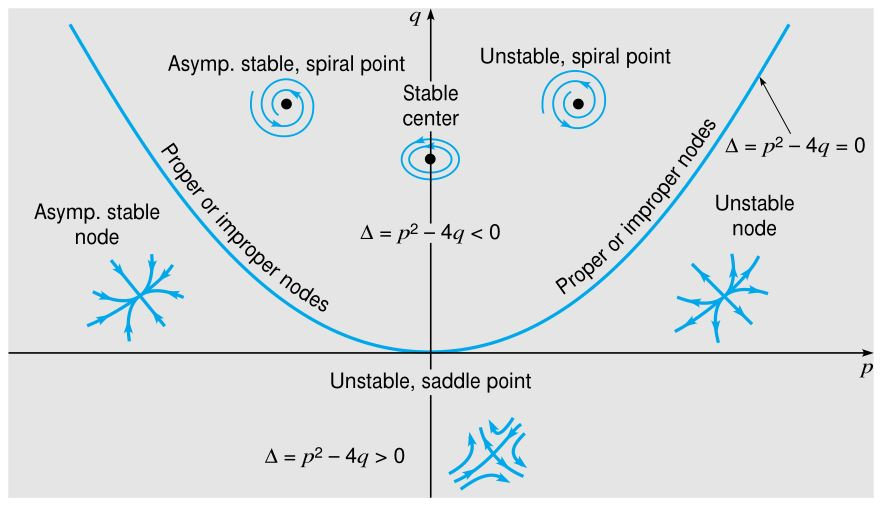
\includegraphics[width=15cm]{phase}
	\\
	Here's a dope diagram, just stare at it for like a long time...  \\
	